\section{Galimi kodo skirstymo į paketus šablonai}
Diskusijose, kaip reikėtų skirstyti programini kodą, paprastai akcentuojami du šablonai - pagal \textit{techninį sluoksnį}, todo: šaltiniai, nurodantys skirstymo būdus
kur kiekvienam funkcionalumui arba kompiuterinės sistemos sluoksniui yra sukuriamas paketas,
grupuojant skirtingų dalykinių sričių esybes, arba pagal \textit{dalykinės srities esybes}, kur vienos esybės kodas, dalykinės srities
esybės funkcionalumas skirtingose programiniuose sluoksniuose yra patalpintas viename pakete.
Tačiau šie du šablonai yra gan platūs ir galėtų būti išskaidyti į daugiau smulkesnių ir tiksliau aprašytų šablonų.
Taip pat, minėtuose šablonuose, būdai kaip ir kodėl skaidyti programinį kodą parinkti akecentuojant tai, kaip programinį
kodą supranta žmonės, dirbantys prie to kodo.
Nuspresti, kaip žmones supranta programinį kodą yra gan sudėtingas ir subjektyvus procesas, todėl aprašant šablonus, kodo skirstymui
geriau akcentuoti, kaip sugrupuoti paketai bendrauja tarpusavyje ir skirstyti juos pagal klasių naudojimo atvejus ir priklausomybes.
Taip kodo grupavimo metodai yra labiau artimi Martino aprašytiems principams.


Šablonus kaip grupuoti kodą, akcentuojant klasių naudojimo atvejus ir priklausomybes nagrinėja Martin Sandin savo
straipsnyje \textit{Four Strategies for Organizing Code}.
Šis straipsnis idomus tuo, kad autorius nesiplečia į du dažniausiai sutiknamus šablonus - grupuoti pagal techninį sluoksni arba dalykinės srities esybes,
o aprašo keturis grupavimo būdus arba šablonus, kurie, nors ir įkvėpti minėtų dviejų budų, yra gan unikalūs ir labiau techniškai apibrėžti.
\subsection{Pagal komponentą}
Organizavimas pagal komponentus sumažina sistemos sudėtingumą, pabrėždamas išorinę ir vidinę kodo vienetų darną.
Išorinė darna reiškia, kad paketas turi minimalią sąsają \angl(interface), kuri atskleidžia tik konceptus (metodus arba duomenų tipus),
kurie yra glaudžiai susijusios su komponento teikiama paslauga.
Vidinė darna reiškia, kad pakuotėje esantis kodas yra stipriai susijęs tarpusavyje ir susijęs su teikiama paslauga.

Kodas yra grupuojamas į mažus paketus, turinčius vieną, aiškiai apibrėžtą funkcionalumą ar tikslą, aprašant abstrakciją, kokie paketo elementai
yra pasiekiami iš išorės ir kaip jie naudojami.
Taip sukuriamas kodas, kuris yra lengviau suprantamas.
Tokį kodo grupavimo tcarką sunku palaikyti, tačiau jo rezultatas - kodas kuris yra lengviau suprantamas, lengviau pagerinamas, lengviau testuojamas
ir, dėl aiškiai aprašytų sąsajų, lengviau pernaudojamas.

\begin{figure}[H]
    \centering
    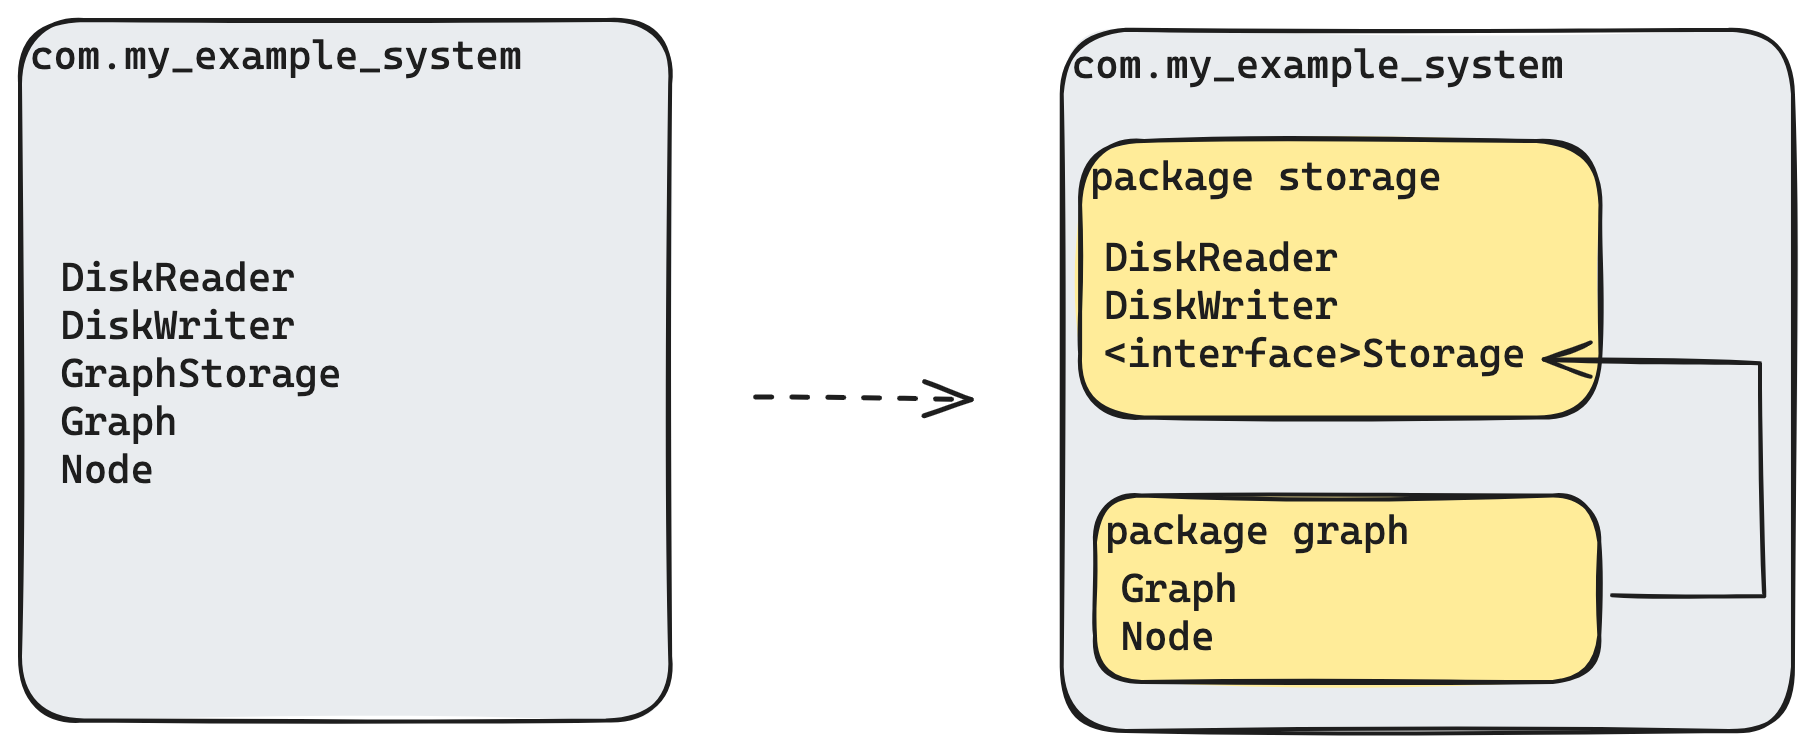
\includegraphics[scale=0.2]{img/component_packaging}
    \caption{Sistemos sugrupuotos pagal komponentą pavizdys}
    \label{img:component_packaging}
\end{figure}
todo: paaiskinti kad cia kaip pagal domeno tipa


\subsection{Pagal techninį sluoksnį}
\subsection{Pagal tipą}